\section{Example Domains}
To demonstrate the efficacy of these approximate abstraction functions, we test functions in the $\ep{Q^*}$ abstraction family on four domains -- NChain, Taxi, Minefield and Random MDP, which we dub ``Random". These domains were selected for their variety -- NChain is relatively simple, Taxi is goal-based and hierarchical in nature, Minefield is stochastic, and Random MDP has many near-optimal policies.

% Description of visuals.
Our code base provides implementations to abstract, visualize, and evaluate an arbitrary MDP to promote further investigation into approximate abstraction. The included visuals of compressed MDPs always converts MDPs into a graph so that an arbitrary MDP may be visualized when abstracted. We use the graph visualization library GraphStream~\cite{graphstream}. In our visuals, a grey circle indicates a state, while the colored arrows indicate transitions. The thickness of the arrow indicates how much reward is associated with that transition. In the ground MDPs, states are labeled with a number. In some abstract MDPs, we indicate which ground states were collapsed to each abstract state by labelling the abstract states with their constituent ground states (some are visually unwieldy and so were ignored).

% Subsection: NChain.
\subsection{NChain}

NChain, pictured in Figure~\ref{fig:nchain-visual}, is a simple MDP heavily investigated in the Bayesian Reinforcement Learning literature due to the interesting exploration problem it poses~\cite{dearden1998bayesian}. In all states, the agent has two actions available: advance down the chain, or return to state 0. The agent receives a small positive reward, $r_{small}$ for returning to state 0, and no reward for advancing down the chain, unless the agent transitions to the last state in the chain. This transition provides a large positive reward, $r_{large}$. Thus, the agent must explore down the chain and avoid the intermediate smaller rewards in order to find the large reward at the end. Transitions also have small slip probability such that the applied action has the unintended effect of the opposing action (so advancing down the chain with probability $\rho$ will take the agent back to state 0, and vice versa). In our implementation, we set $N=10$, $\rho=0.2$, $r_{small} = 0.2$, and $r_{large} = 1.0$.

% NChain Compression Visuals.
\begin{figure}[h]
\subfigure[Ground NChain]{
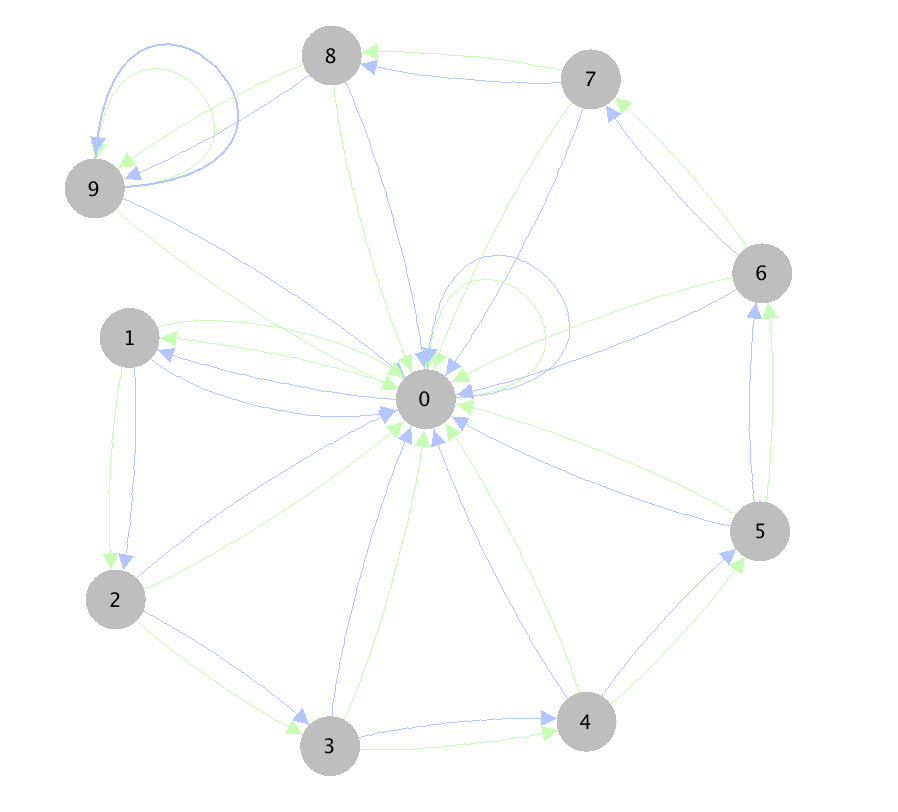
\includegraphics[width=0.48\columnwidth]{figures/ground_nchain.png}}
\subfigure[Abstract NChain]{
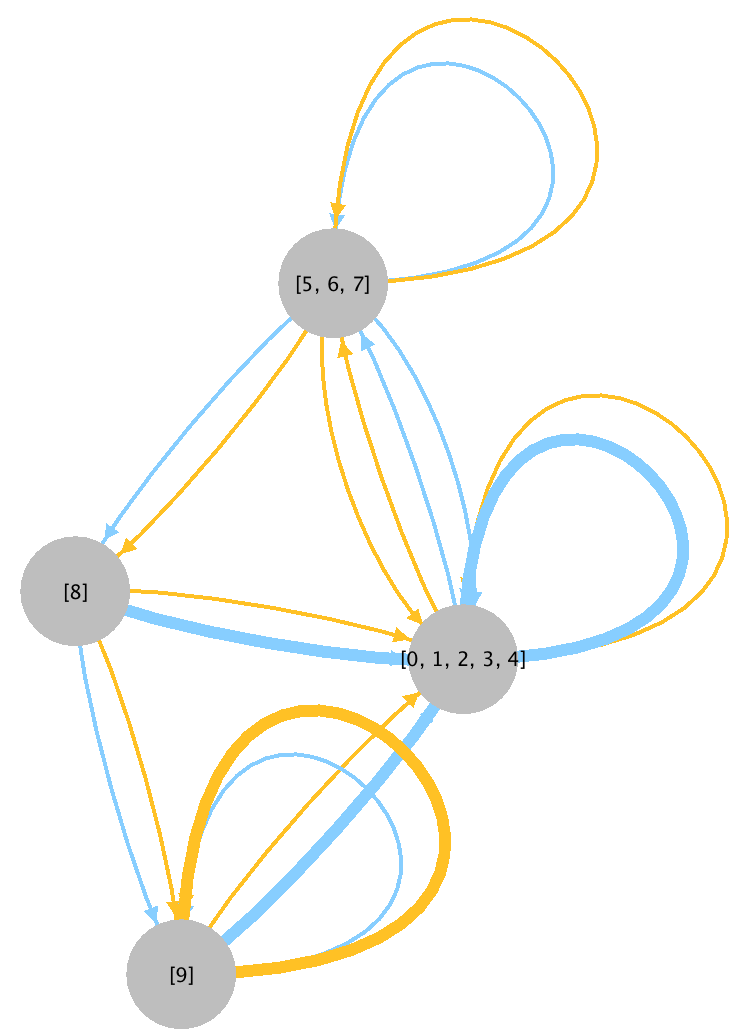
\includegraphics[width=0.48\columnwidth]{figures/abs_nchain.png}}
\label{fig:nchain-visual}
\caption{Comparison of Original NChain MDP and Abstract NChain MDP, under an $\epQ$ abstraction, with $\epsilon=0.5$}
\end{figure} 

%% Subsection: UpWorld.
%\subsection{UpWorld}
%
%The UpWorld task is an $N\times M$ grid in which the agent starts in the lower left corner. The agent may move left, right, and up. The agent receives positive reward for transitioning to a state at the top of the grid, where moving up in the top cells self transitions. the agent receives 0 reward for all other transitions. Consequently, moving up is always the optimal action, since moving left and right does not change the agent's manhattan distance to positive reward. During experimentation, we set $N=10$, $M=4$.
%
%\begin{figure}
%\subfigure[Ground UpWorld]{
%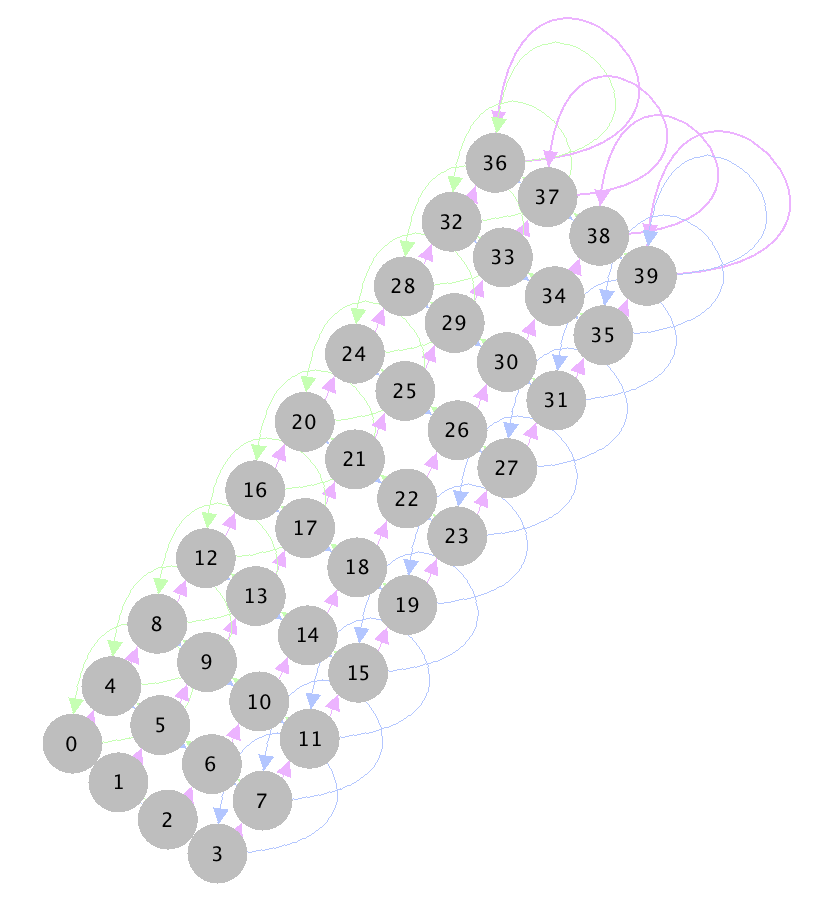
\includegraphics[width=0.48\columnwidth]{figures/ground_upworld.png}}
%\subfigure[Abstract UpWorld]{
%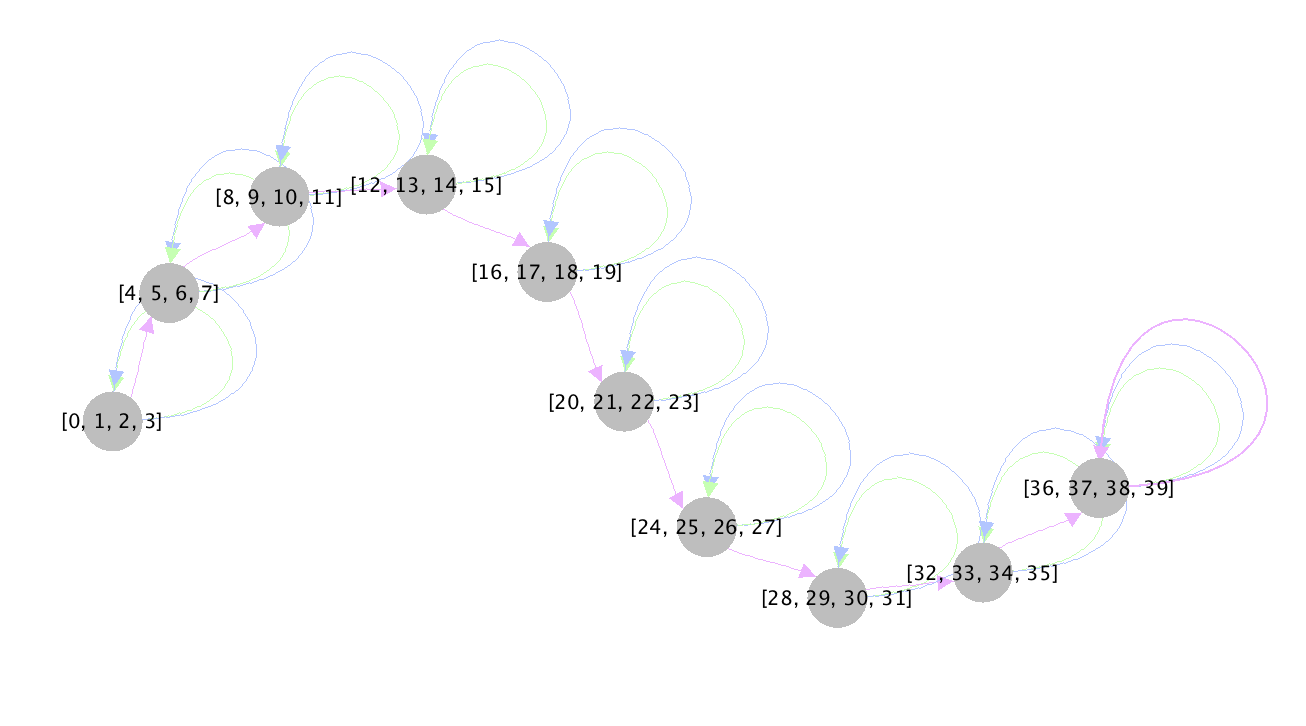
\includegraphics[width=0.48\columnwidth]{figures/abs_upworld.png}}
%\label{fig:upworld-visual}
%\caption{Comparison of Original UpWorld MDP and Abstract MDP, under $\epQ$, with $\epsilon=0.5$}
%\end{figure} 

% Subsection: Taxi
\subsection{Taxi}

Taxi has long been studied by the hierarchical reinforcement learning literature due to its natural decomposition into hierarchical subgoals~\cite{dietterich2000hierarchical}. The agent, operating in a grid world style domain, may move left, right, up, and down, as well as pickup a passenger and drop off a passenger. The goal is achieved when the agent has taken each passenger to its destination.

%We visualize the compression on a simple 626 Taxi instance in Figure~\ref{fig:taxi-visual}. As stated above, we visualize the original Taxi problem into a graph representation so that we may visualize both the ground MDP and abstract MDP in the same format.

% Taxi Compression Visuals
%\begin{figure}[h]
%\subfigure[Ground Taxi]{
%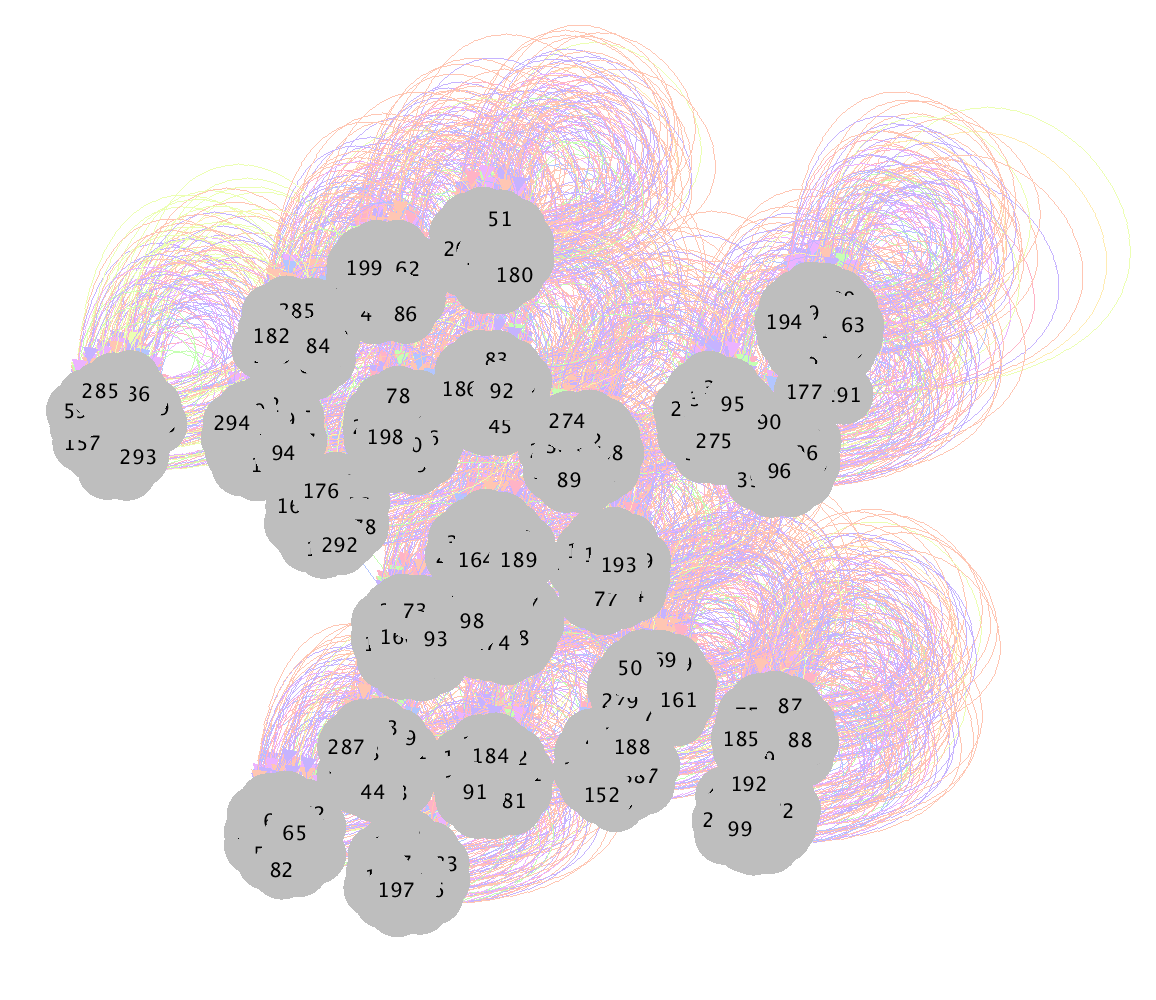
\includegraphics[width=0.48\columnwidth]{figures/ground_taxi.png}}
%\subfigure[Abstract Taxi]{
%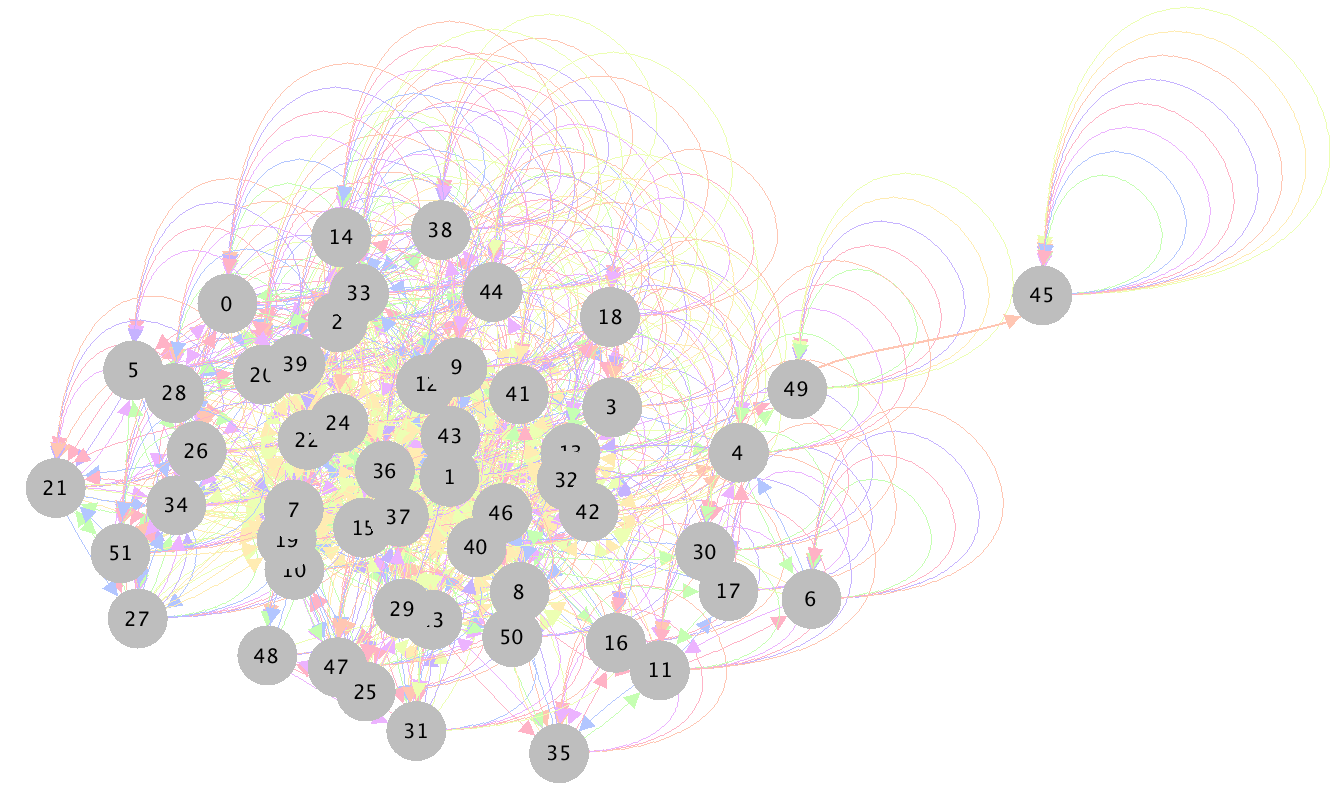
\includegraphics[width=0.48\columnwidth]{figures/abs_taxi.png}}
%\label{fig:taxi-visual}
%\caption{Comparison of Original Taxi MDP and Abstract Taxi MDP, under an $\epQ$ abstraction, with $\epsilon=0.03$}
%\end{figure} 


% Insert visual and/or stats on number of states and performance of VI solving the abstract MDP and evaluating the resulting policy on the original MDP


% Subsection: Minefield.
\subsection{Minefield}

Minefield is a slight variant of Grid World. The transitions and rewards are perturbed, and there is no down action available to the agent. There is some slip probability associated with movement; when the agent moves left or right, it has probability $x$ of moving up, when the agent moves up, it has probability $\frac{x}{2}$ of moving left, and probability $\frac{x}{2}$ of moving right. The reward function is such that transitions to the top row in the grid receive $1.0$ reward, all other transitions receive $0.2$ reward, except for a random set of $\kappa$ states (which may include the top row) that receive $0$ reward (these are the states with mines in them, thus the name). During experimentation, we set $N=10, M=4, \epsilon=1.1, \kappa = 5, x = 0.01$. We visualize the original Minefield, represented as a graph, and the abstract Minefield in ~\ref{ref:minefield-visual}.

% Minefield Compression Visuals
\begin{figure}
\subfigure[Ground Minefield]{
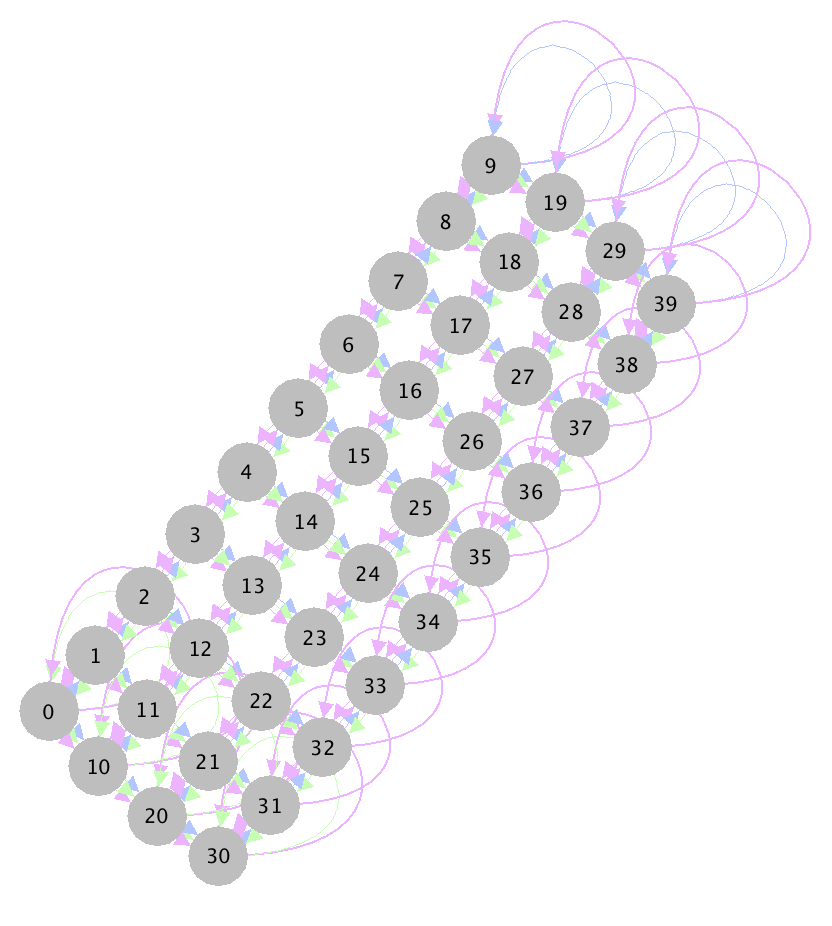
\includegraphics[width=0.48\columnwidth]{figures/ground_minefield.png}}
\subfigure[Abstract Minefield]{
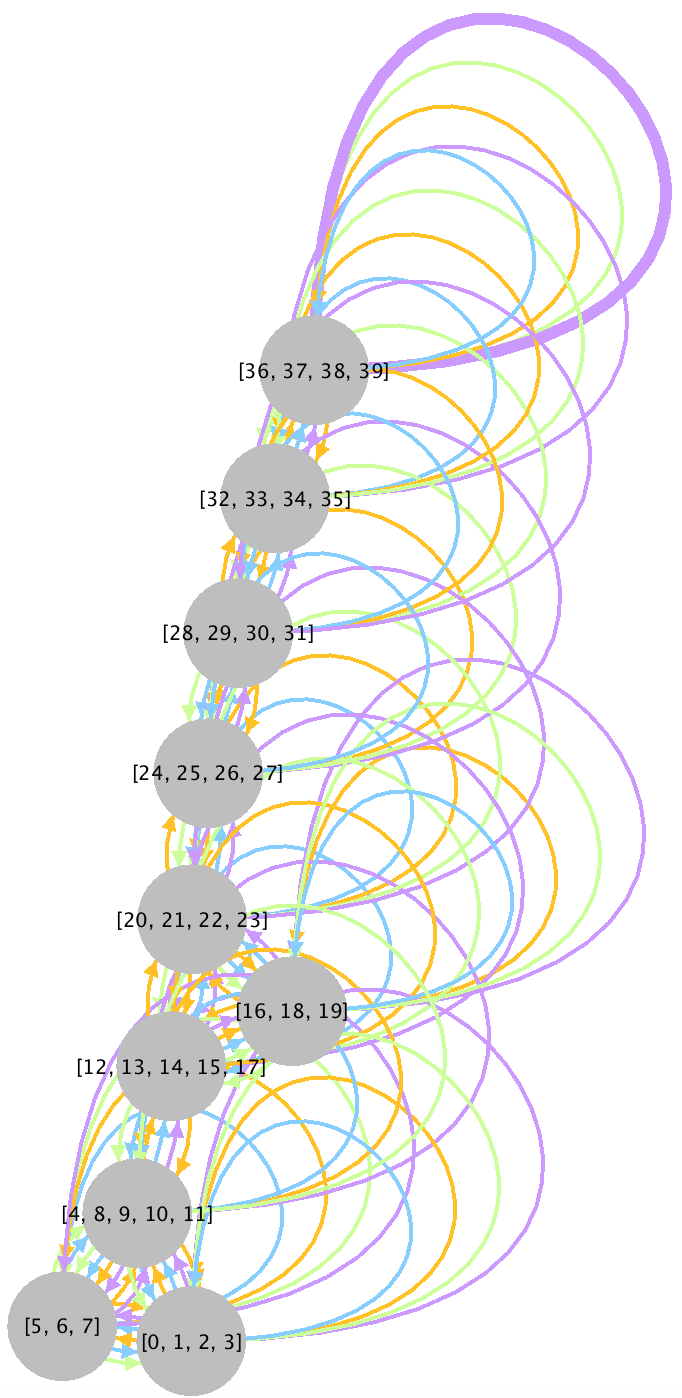
\includegraphics[width=0.48\columnwidth]{figures/abs_minefield.png}}
\label{fig:minefield-visual}
\caption{Comparison of Original Minefield MDP and Abstract MDP, under an $\epQ$ abstraction, with $\epsilon=1.1$}
\end{figure} 


% Subsection: Random.
\subsection{Random}

The Random MDP domain we consider is as follows. There are $N$ states, and $K$ actions. For each state, each action can transition to two randomly selected (but fixed) states, each with probability $0.5$.

%The Random MDP and its compression are visualized in Figure~\ref{fig:minefield-visual}.

% Random Compression Visuals
%\begin{figure}
%\subfigure[Ground Random]{
%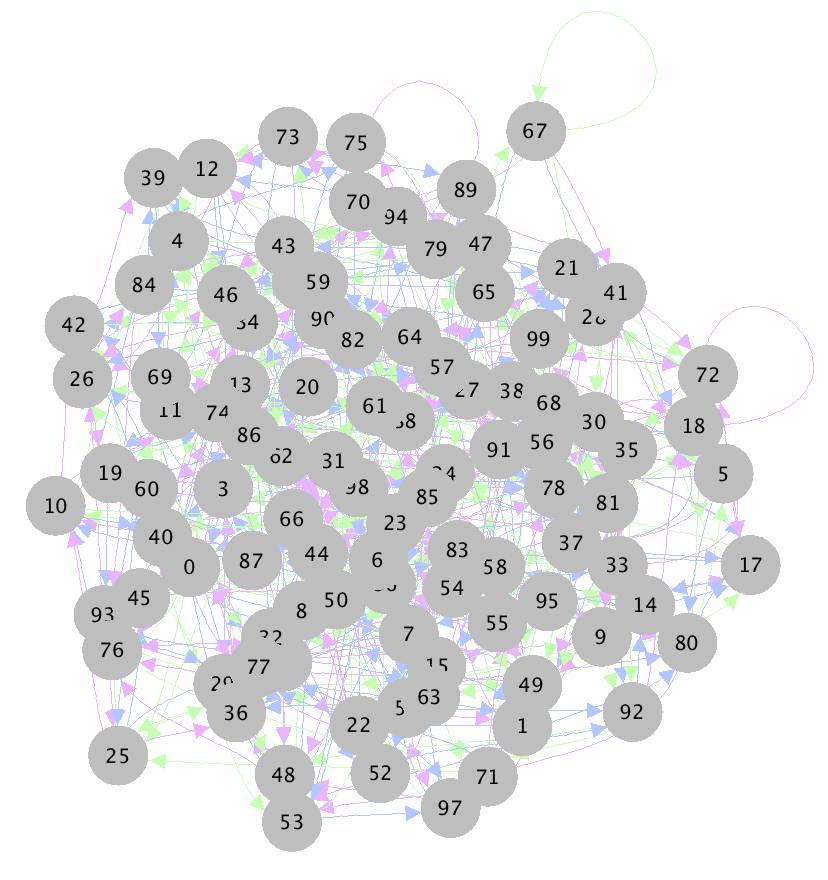
\includegraphics[width=0.48\columnwidth]{figures/ground_random.png}}
%\subfigure[Abstract Random]{
%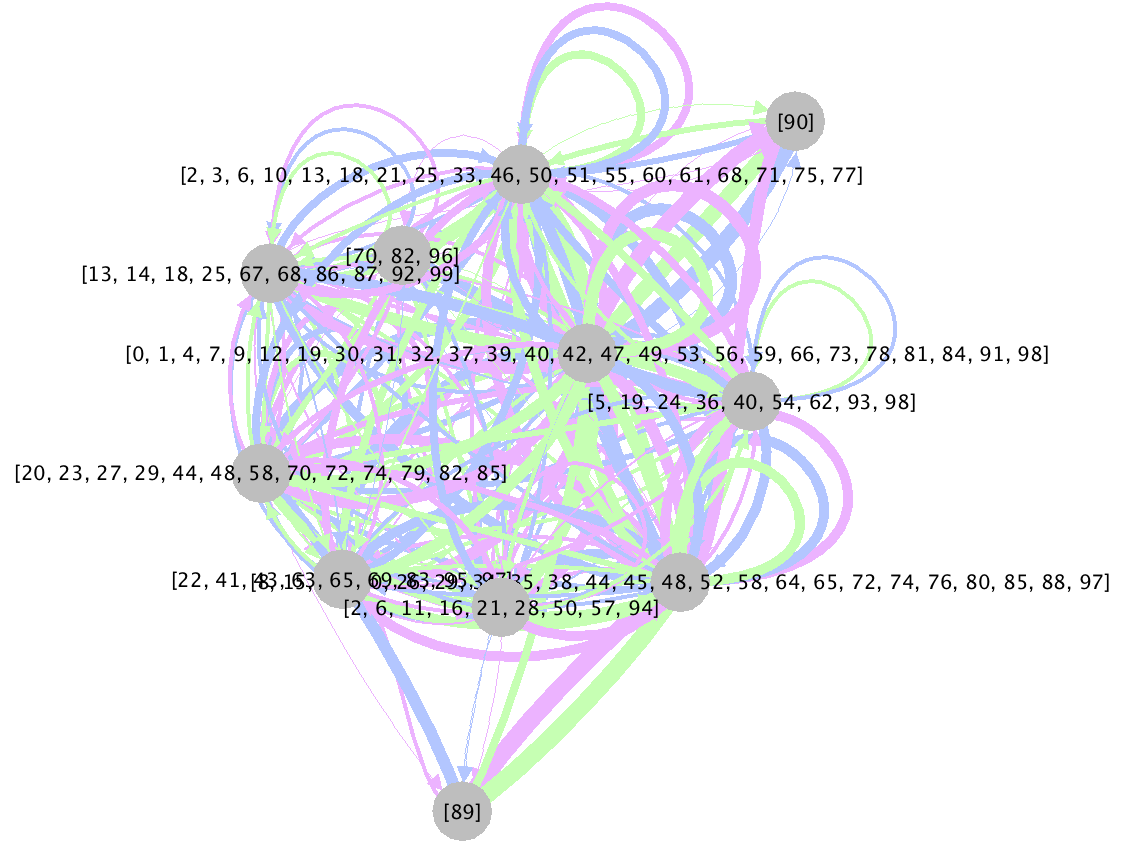
\includegraphics[width=0.48\columnwidth]{figures/abs_random.png}}
%\label{fig:minefield-visual}
%\caption{Comparison of Original Random MDP and Abstract Random MDP, under an $\epQ$ abstraction, with $\epsilon=0.2$}
%\end{figure} 
